\documentclass{article}
\usepackage[utf8]{inputenc}
\usepackage[spanish]{babel}
\usepackage{amsmath}
\usepackage{amssymb}
\usepackage{amsthm}
\usepackage{graphicx}
\usepackage{float}
\usepackage{listings}
\usepackage{xcolor}
\usepackage{geometry}

\geometry{margin=2.5cm}

% Entornos tipo teorema (amsthm)
\theoremstyle{plain}
\newtheorem{theorem}{Teorema}
\theoremstyle{definition}
\newtheorem{definition}{Definición}

% Configuración para mostrar código (Python)
\lstset{
    language=Python,
    basicstyle=\ttfamily\small,
    keywordstyle=\color{blue}\bfseries,
    commentstyle=\color{green!60!black}\itshape,
    stringstyle=\color{red!70!black},
    numbers=left,
    numberstyle=\tiny\color{gray},
    stepnumber=1,
    numbersep=8pt,
    backgroundcolor=\color{gray!5},
    frame=single,
    rulecolor=\color{black!30},
    breaklines=true,
    breakatwhitespace=false,
    tabsize=4,
    captionpos=b,
    xleftmargin=1.5em,
    framexleftmargin=1.2em,
    showstringspaces=false
}

\title{Memoria en Distribuciones y Propiedad Sin Memoria: Caso Exponencial}
\author{Juan Felipe Rodr\'iguez G. (20261595004)}
\date{\today}

\begin{document}
\maketitle

\section*{Contexto del Problema}

En probabilidad, muchas variables aleatorias modelan \emph{tiempos de espera} (por ejemplo: tiempo hasta que falle un componente, tiempo hasta que llegue un paquete o tiempo hasta que ocurra un evento). En estos contextos surge una pregunta natural:

\begin{quote}
\emph{Si ya ha transcurrido cierto tiempo sin que ocurra el evento, \textquestiondown eso cambia la probabilidad de seguir esperando?}
\end{quote}

A esta idea se le suele llamar \textbf{``memoria''} de una distribución. La tarea solicita:
\begin{enumerate}
    \item Explicar el concepto de memoria.
    \item Determinar si la distribución exponencial no tiene memoria.
    \item Determinar si la exponencial es la \emph{única} distribución continua sin memoria.
\end{enumerate}

\section*{Concepto de ``memoria'' en una distribución}

Sea $T$ una variable aleatoria no negativa que representa un tiempo de espera. Decimos informalmente que la distribución de $T$ \textbf{tiene memoria} cuando el tiempo ya transcurrido afecta la distribución del tiempo restante.

Formalmente, el tiempo restante después de haber esperado $s$ unidades es:
$$ (T - s) \ \text{condicionado a que } T > s. $$

Si la distribución \emph{no} tiene memoria, entonces el tiempo restante se comporta como si el proceso \emph{acabara de comenzar}. Es decir, la información \(T > s\) no cambia la ley del tiempo adicional a esperar.

\section*{Definición matemática de la propiedad sin memoria}

\begin{definition}[Propiedad sin memoria]
Una variable aleatoria no negativa $T$ es \textbf{sin memoria} si para todo $s,t \ge 0$ se cumple:
\begin{equation} \label{eq:memoryless}
P(T > s+t \mid T > s) = P(T > t).
\end{equation}
\end{definition}

Esta identidad dice: \emph{``si ya esperé $s$ y todavía no pasa nada, la probabilidad de esperar al menos $t$ más es la misma que al inicio''}.

\subsection*{Reescritura con la función de supervivencia}

Definimos la función de supervivencia (o cola) como:
$$ S(t) = P(T > t). $$

Usando la definición de probabilidad condicional, la ecuación (\ref{eq:memoryless}) se transforma en:
\begin{align*}
P(T > s+t \mid T > s)
&= \frac{P(T > s+t \cap T > s)}{P(T > s)} \\
&= \frac{P(T > s+t)}{P(T > s)}
= \frac{S(s+t)}{S(s)}.
\end{align*}

Por tanto, $T$ es sin memoria si y solo si:
\begin{equation} \label{eq:survival_cauchy}
S(s+t) = S(s)\,S(t), \quad \forall\, s,t \ge 0.
\end{equation}

\section*{\textquestiondown Es cierto que la distribución exponencial no tiene memoria?}

\subsection*{Recordatorio: distribución exponencial}

Decimos que $T \sim \mathrm{Exp}(\lambda)$ (con $\lambda > 0$) si su densidad es:
$$ f(t) = \lambda e^{-\lambda t}, \quad t \ge 0. $$

Su función de supervivencia es:
\begin{equation} \label{eq:exp_survival}
S(t) = P(T > t) = e^{-\lambda t}.
\end{equation}

\subsection*{Demostración de que es sin memoria}

Tomando $S(t)$ de (\ref{eq:exp_survival}), para $s,t \ge 0$:
\begin{align*}
S(s+t)
&= e^{-\lambda(s+t)} \\
&= e^{-\lambda s}\, e^{-\lambda t}
= S(s)\,S(t).
\end{align*}

Esto coincide exactamente con la condición (\ref{eq:survival_cauchy}). Por tanto:
\begin{equation*}
P(T > s+t \mid T > s) = P(T > t).
\end{equation*}

\begin{flushright}
\qedsymbol
\end{flushright}

\textbf{Conclusión parcial:} Sí, \textbf{la distribución exponencial no tiene memoria}.

\section*{\textquestiondown Es cierto que la exponencial es la única distribución continua sin memoria?}

La respuesta (bajo supuestos estándar de continuidad) también es \textbf{sí}: la exponencial es la única distribución continua \emph{no degenerada} en $[0,\infty)$ que satisface la propiedad sin memoria.

\begin{theorem}[Unicidad de la exponencial]
Sea $T$ una variable aleatoria continua no negativa con función de supervivencia $S(t) = P(T>t)$. Si $S$ satisface
$$ S(s+t) = S(s)\,S(t) \quad \forall\, s,t \ge 0, $$
además de ser continua y con $S(0)=1$, entonces existe $\lambda \ge 0$ tal que:
$$ S(t) = e^{-\lambda t} \quad (t\ge 0). $$
En particular, si $\lambda>0$, entonces $T \sim \mathrm{Exp}(\lambda)$.
\end{theorem}

\subsection*{Demostración (idea central)}

Partimos de la ecuación funcional (\ref{eq:survival_cauchy}). Observamos primero que $S(0)=P(T>0)=1$ y que $0 \le S(t) \le 1$.

Si definimos:
$$ g(t) = -\ln(S(t)), $$
entonces la ecuación $S(s+t)=S(s)S(t)$ se convierte en:
\begin{align*}
-\ln(S(s+t)) &= -\ln(S(s)S(t)) \\
g(s+t) &= g(s) + g(t).
\end{align*}

La última ecuación es la ecuación aditiva de Cauchy. Como $g$ hereda continuidad (porque $S$ es continua y $S(t)>0$), se concluye que:
$$ g(t) = \lambda t \quad \text{para algún } \lambda \ge 0. $$

Por lo tanto:
$$ S(t) = e^{-g(t)} = e^{-\lambda t}, $$
que es exactamente la supervivencia de una exponencial. 

\begin{flushright}
\qedsymbol
\end{flushright}

\textbf{Conclusión final:} Sí, \textbf{la distribución exponencial es la única distribución continua sin memoria} (exceptuando el caso degenerado $P(T=0)=1$, que no es útil como modelo de espera).

\section*{Comentario (conexión con distribuciones discretas)}

En el mundo \textbf{discreto}, la análoga sin memoria no es la exponencial sino la \textbf{geométrica}. Esta observación es útil para entender que la propiedad sin memoria es muy restrictiva: básicamente ``selecciona'' una familia específica dependiendo de si el tiempo se mide continuo o en pasos.

\section*{Comprobación por simulación (Python, opcional)}

Se puede \emph{comprobar por simulación} la igualdad
$$ P(T > s+t \mid T > s) \approx P(T > t) $$
cuando $T \sim \mathrm{Exp}(\lambda)$, usando Monte Carlo, en este caso utilizando python.

\begin{lstlisting}[caption={Script de simulación: comprobación empírica de la propiedad sin memoria (Exponencial)}]
# simulacion_memoria_exponencial.py
# Ejecutar: python3 simulacion_memoria_exponencial.py

import random
import math


def estimar_probabilidades(lmbda: float, s: float, t: float, n: int = 200000):
    """Estima P(T>s+t | T>s) y P(T>t) para T~Exp(lambda)."""
    count_gt_s = 0
    count_gt_s_and_gt_s_plus_t = 0
    count_gt_t = 0

    for _ in range(n):
        # random.expovariate(lmbda) genera una Exp(lambda)
        T = random.expovariate(lmbda)

        if T > s:
            count_gt_s += 1
            if T > s + t:
                count_gt_s_and_gt_s_plus_t += 1

        if T > t:
            count_gt_t += 1

    p_cond = count_gt_s_and_gt_s_plus_t / count_gt_s
    p_tail = count_gt_t / n

    # Valores teoricos
    p_cond_teo = math.exp(-lmbda * t)
    p_tail_teo = math.exp(-lmbda * t)

    return p_cond, p_tail, p_cond_teo, p_tail_teo


if __name__ == "__main__":
    lmbda = 2.0
    s = 1.5
    t = 0.75

    p_cond, p_tail, p_cond_teo, p_tail_teo = estimar_probabilidades(lmbda, s, t)

    print("=== Exponencial sin memoria (simulacion) ===")
    print(f"lambda = {lmbda}, s = {s}, t = {t}")
    print(f"Estimado  P(T>s+t | T>s) = {p_cond:.5f}")
    print(f"Estimado  P(T>t)         = {p_tail:.5f}")
    print(f"Teorico   exp(-lambda t) = {p_cond_teo:.5f}")
\end{lstlisting}

\textbf{Qué se espera observar:} ambos estimados (condicional y cola) quedan muy cercanos entre sí y al valor teórico $e^{-\lambda t}$; pequeñas diferencias se deben al error Monte Carlo.

\begin{figure}[H]
    \centering
    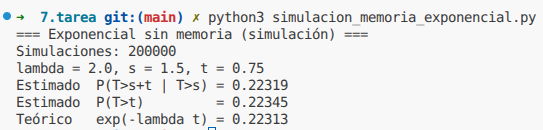
\includegraphics[width=0.55\textwidth]{captura_script_python.png}
    \caption{Pantallazo de ejecución del script de comprobación en Python. Se observa que $P(T>s+t\mid T>s)$ y $P(T>t)$ son muy cercanas y además se aproximan a $e^{-\lambda t}$.}
    \label{fig:pantallazo-python}
\end{figure}

\section*{Conclusiones}

\begin{itemize}
    \item ``Memoria'' significa que el tiempo ya transcurrido cambia la distribución del tiempo restante.
    \item La propiedad sin memoria se formaliza como $P(T>s+t\mid T>s)=P(T>t)$.
    \item La distribución exponencial cumple esta propiedad.
    \item Bajo continuidad, la ecuación funcional $S(s+t)=S(s)S(t)$ fuerza a que $S(t)=e^{-\lambda t}$, por lo que la exponencial es la única distribución continua sin memoria.
\end{itemize}

\begin{thebibliography}{}

\bibitem{walpole2017}
Walpole, R. E., Myers, R. H., Myers, S. L., \& Ye, K. (2017).
\textit{Probability and Statistics for Engineers and Scientists} (9th ed.).
Pearson.

\end{thebibliography}

\end{document}
